\chapter{Troubleshooting}

\section{Documentation}

For network administrators to be able to monitor and troubleshoot a network, they must have a complete set of accurate and current network documentation. This documentation includes:

\begin{itemize}
\item Configuration files, including network configuration files and end-system configuration files
\item Physical and logical topology diagrams 
\item A network baseline 
\end{itemize}

\subsection{Configuration files}

Network configuration files contain accurate, up-to-date records of the hardware (routers, switches, cables etc.) and software (routing protocols, IOS, etc.) used in a network. End-system configuration files focus on the hardware and software used in end-system devices, such as servers, network management consoles, and user workstations. See also figures \ref{Configuration} and \ref{EndSystem}.

\begin{figure}[hbtp]
\caption{Network configuration file}\label{Configuration}
\centering
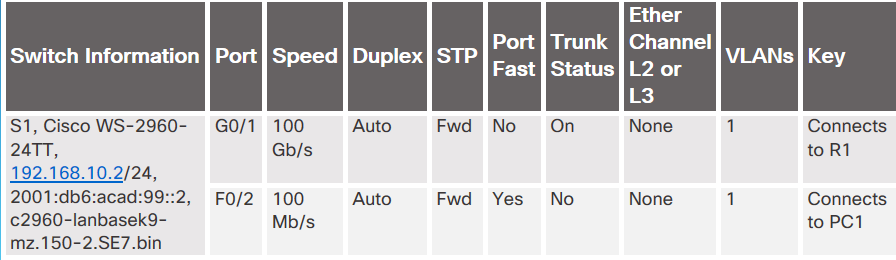
\includegraphics[ width=0.8\textwidth ]{pictures/Configuration.PNG}
\end{figure}

\begin{figure}[hbtp]
\caption{End-system configuration file}\label{EndSystem}
\centering
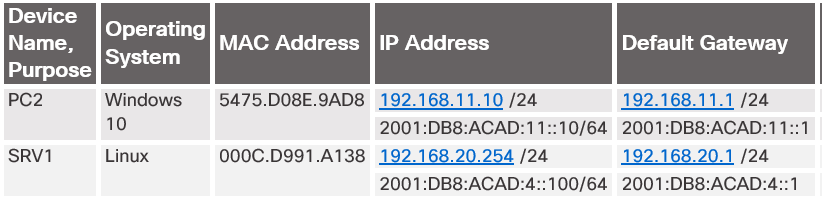
\includegraphics[ width=0.8\textwidth ]{pictures/EndSystem.PNG}
\end{figure}

\subsection{Topology diagrams}

There are two types of network topology diagrams: the physical topology and the logical topology. A physical network topology shows the physical layout of the devices connected to the network. It is useful when troubleshooting physical layer problems. A logical network topology illustrates how devices are logically connected to the network, meaning how devices actually transfer data across the network when communicating with other devices. Symbols are used to represent network elements.

\subsection{Network baseline}

A baseline is used to establish normal network or system performance. Establishing a network performance baseline requires collecting performance data from the ports and devices that are essential to network operation. A network baseline helps:

\begin{itemize}
\item monitor network behavior
\item keep track of the performance
\item keep track of the traffic patterns
\item check whether the current network design can meet business requirements
\item measure the optimum nature of network traffic and congestion levels
\item show the true nature of congestion or potential congestion in a network
\item reveal areas in the network that are underutilized 
\end{itemize}

To establish and capture an initial network baseline, perform the following steps:

\begin{enumerate}
\item Determine what types of data to collect
\item Identify devices and ports of interest
\item Determine the baseline duration (a baseline needs to last no more than six weeks, a two-to-four-week baseline is adequate.)
\end{enumerate}

Baseline measurements should not be performed during times of unique traffic patterns, because the data would provide an inaccurate picture of normal network operations. Baseline analysis of the network should be conducted on a regular basis. Perform an annual analysis of the entire network or different sections of the network on a rotating basis. Analysis must be conducted regularly to understand how the network is affected by growth and other changes.

\section{Troubleshooting process}

\subsection{General procedures}

\begin{enumerate}
\item \textbf{Gather symptoms:} the network administrator determines which network components have been affected and how the functionality of the network has changed compared to the baseline.
\item \textbf{Isolate the problem:}  Isolating is the process of eliminating variables until a single problem, or a set of related problems has been identified as the cause.
\item \textbf{Implement corrective action:} implementing, testing, and documenting possible solutions.
\end{enumerate}

\subsubsection{Gathering symptoms}

There are five information gathering steps:

\begin{enumerate}
\item \textbf{Gather information:} Get information from trouble ticket or questioning users. Table \ref{tab:questioning} provides some guidelines and sample end-user question.
\item \textbf{Determine ownership:} If the problem is outside the boundary of the organization's control, contact an administrator for the external system.
\item \textbf{Narrow the scope:} Determine in which layer the problem occurs (core, distribution, or access layer).
\item \textbf{Gather symptoms from suspect devices:} Use a layered troubleshooting approach and Gather hardware and software symptoms. To gather symptoms, use Cisco IOS commands (ping, traceroute, telnet, show, debug) or packet captures, device logs.
\item \textbf{Document symptoms} 
\end{enumerate}

\begin{table}[hbtp]\label{tab:questioning}
\centering
\begin{tabular}{ p{0.4\textwidth} p{0.4\textwidth} }
\toprule
\head{Guidelines} & \head{Sample questions}\\
\midrule
Ask questions that are pertinent to the problem & What does not work? \\
Questions that help eliminate or discover the possible problems & Are things that do work and the things that do not work related? \\
Speak at technical level that the user can understand & Has the thing that does not work ever worked? \\
Ask the user when the problem was first noticed & When was the problem first noticed? \\
Determine whether anything unusual since the last time it worked & What has changed since the last time it did work? \\
Recreate the problem & Can you reproduce the problem? \\
What happened before the problem occurred & When exactly does the problem occur?\\
\bottomrule
\end{tabular}
\end{table}

\subsubsection{Implement corrective action}

The severity of the problem should be weighed against the impact of the solution. For example, if a critical server or router must be offline for a significant amount of time, it may be better to wait until the end of the workday to implement the fix. This is called \textbf{change-control procedures}.\\

If the corrective action creates another problem or does not solve the problem, the attempted solution is documented, the changes are removed, and the network administrator returns to gathering symptoms and isolating the issue.

\subsection{Troubleshooting methods}

\paragraph{Bottom-up}you start with the physical components of the network and move up through the layers of the OSI model until the cause of the problem is identified. Bottom-up troubleshooting is a good approach to use when the problem is suspected to be a physical one.\\

\paragraph{Top-down}starts with the end-user applications and moves down through the layers of the OSI model until the cause of the problem has been identified. Use this approach for simpler problems, or when you think the problem is with a piece of software. The disadvantage with the top-down approach is it requires checking every network application until the possible cause of the problem is found.

\paragraph{Divide-conquer}The network administrator selects a layer and tests in both directions from that layer. You make an informed guess as to which OSI layer to start your investigation. When a layer is verified to be functioning properly, it can be assumed that the layers below it are functioning. The administrator can work up the OSI layers. If an OSI layer is not functioning properly, the administrator can work down the OSI layer model.

\paragraph{Educated guess}The network administrator guesses the solution based on the symptoms of the problem. This method is more successfully implemented by seasoned network administrators, because seasoned network administrators rely on their extensive knowledge and experience to decisively isolate and solve network issues. 

\paragraph{Comparison}Comparing a working to a non-working situation involves comparing configurations, software versions, and hardware changes. The aim is to identify the changes that led to a non-working environment. Using this method may lead to a working solution, but without clearly revealing the cause of the problem. This method can be helpful when the network administrator is lacking an area of expertise, or when the problem needs to be resolved quickly. After the fix has been implemented, the network administrator can do further research on the actual cause of the problem.

\paragraph{Substitution}involves swapping the problematic device with a known, working one. If the problem is fixed, that the network administrator knows the problem is with the removed device. If the problem remains, then the cause may be elsewhere. In specific situations, this can be an ideal method for quick problem resolution.

\section{Using IP SLA}

\subsection{Introduction}

Network engineers use IP SLAs to simulate network data and IP services to collect network performance information in real time. Multiple IP SLA operations may be configured on a device. There are additional benefits for using IP SLAs: 

\begin{itemize}
\item Service-level agreement monitoring, measurement, and verification
\item Network performance monitoring
\item IP service network health assessment to verify that the existing QoS is sufficient for IP services
\item Edge-to-edge network availability monitoring for proactive connectivity verification of network resources
\end{itemize}

Instead of using ping manually, a network engineer can use the IP SLA ICMP Echo operation to test the availability of network devices. The IP SLA ICMP Echo operation provides the following measurements:

\begin{itemize}
\item Availability monitoring (packet loss statistics)
\item Performance monitoring (latency and response time)
\item Network operation (end-to-end connectivity)
\end{itemize}

\subsection{Configuration}

To create an IP SLA operation and enter IP SLA configuration mode, use the \verb|ip sla <operation-number>| global configuration command. From IP SLA configuration mode, you can configure the IP SLA operation as an ICMP Echo operation and enter ICMP echo configuration mode using the following command:

\begin{verbatim}
Router(config-ip-sla)# icmp-echo { dest-ip-address | dest-hostname } 
						[ source-ip { ip-address | hostname } 
						| source-interface interface-id ] 
\end{verbatim}

Next, set the rate at which a specified IP SLA operation repeats using the \verb|frequency <seconds>| command. To schedule the IP SLA operation, use the following global configuration command:

\begin{verbatim}
Router(config)# ip sla schedule operation-number 
                [ life { forever | seconds }] 
                [ start-time { hh : mm [: ss ] [ month day | day month ] 
                | pending | now | after hh:mm:ss ] [ ageout seconds ] 
                [ recurring ] 
\end{verbatim}

\subsection{Sample}

The configuration below configures an IP SLA operation with an operation number of 1.  Each operation can be referred to by its operation-number. The \verb|icmp-echo| command identifies the destination address to be monitored. The frequency command is setting the IP SLA rate to 30 second intervals. The \verb|ip sla schedule| command is scheduling the IP SLA operation number 1 to start immediately (now) and continue until manually cancelled (forever).

\begin{verbatim}
R1(config)# ip sla 1
R1(config-ip-sla)# icmp-echo 192.168.1.5
R1(config-ip-sla)# frequency 30
R1(config-ip-sla)# exit
R1(config)# ip sla schedule 1 start-time now life forever
\end{verbatim}

\section{Troubleshooting tools}

\subsection{Software}

\paragraph{Network management system (NMS)}includes device-level monitoring, configuration, and fault-management tools.  These tools can be used to investigate and correct network problems.

\paragraph{Knowledge base} is a vendor-based webpage that provides information on hardware and software. It contains troubleshooting procedures, implementation guides, and original white papers on most aspects of networking technology.

\paragraph{Baselining tools}automate  the network documentation and baselining process. For example, they can draw network diagrams, help keep network software and hardware documentation up-to-date, and help to cost-effectively measure baseline network bandwidth use.

\paragraph{Protocol analyzer} useful to investigate packet content while flowing through the network. The information displayed by a protocol analyzer includes the physical, data link, protocol, and descriptions for each frame. Protocol analyzers such as Wireshark can help troubleshoot network performance problems, verify authentication, etc.

\subsection{Hardware}

\paragraph{Digital multimeters (DMMs)}are test instruments that are used to directly measure electrical values of voltage, current, and resistance. We use them to check power supply voltage levels. 

\paragraph{Cable testers} are designed for testing data communication cabling. It can be used to detect broken wires, crossed-over wiring, shorted connections, and improperly paired connections. There is one type of cable testers called time-domain reflectometers (TDRs). These devices are used to pinpoint the distance to break in a cable.

\paragraph{Cable analyzers} are used to test and certify copper and fiber cables. It can detect near-end crosstalk (NEXT), return loss (RL), etc.

\paragraph{Portable network analyzers} are used for troubleshooting VLANs and switched networks. Using this device, the network engineer can view interface details, see which switch port is connected to which device, discover VLAN configuration, analyze network traffic, etc.

\paragraph{Network analysis module (NAM)} provides embedded browser-based interface that generates report on the network resources. NAM can also capture and decode packets, track response time, etc.

\section{Scenarios}

\begin{example}
A network engineer is troubleshooting a network problem where users cannot access the FTP server at the same IP address where a website can be successfully accessed. Which troubleshooting method would be the best to apply in this case? 
\end{example}

\begin{solution}
The fact that some application layer services provided by a network device are operating successfully but others are not means that the lower OSI or TCP/IP layers are functional with the problem likely to be in the application layer. Therefore, the troubleshooting method is \emph{bottom-up}.
\end{solution}

\begin{example}
A network engineer is troubleshooting a network that has recently been updated with a new routing protocol, but the network is not working as expected. The engineer is comparing the running configuration from before and after the change was made. Which approach to troubleshooting the problem is the engineer using? 
\end{example}

\begin{solution}
This is a variation on the divide-and-conquer method. Since a routing protocol change was recently made, the administrator can be fairly certain the issue resides with the network layer.
\end{solution}

\begin{example}
A company is setting up a web site with SSL technology to protect the authentication credentials required to access the web site. A network engineer needs to verify that the setup is correct and that the authentication is indeed encrypted. Which tool should be used?
\end{example}

\begin{solution}
To verify that the authentication is indeed encrypted, the authentication process needs to be captured and investigated, which can be accomplished through a protocol analyzer, such as Wireshark. 
\end{solution}

\begin{example}
A user in a large office calls technical support to complain that a PC has suddenly lost connectivity to the network. The technician asks the caller to talk to nearby users to see if other machines are affected. The caller reports that several immediate neighbors in the same department have a similar problem and that they cannot ping each other. Those who are seated in other departments have connectivity. What should the technician check as the first step in troubleshooting the issue?
\end{example}

\begin{solution}
The status of the departmental workgroup switch in the wiring closet
\end{solution}

\begin{example}
A user reports that after an OS patch of the networking subsystem has been applied to a workstation, it performs very slowly when connecting to network resources. A network technician tests the link with a cable analyzer and notices that the workstation sends an excessive number of frames smaller than 64 bytes and also other meaningless frames. What is the possible cause of the problem?
\end{example}

\begin{solution}
The symptom of excessive runt packets and jabber is typically a Layer 1 issue, such as caused by a corrupted NIC driver, which could be the result of a software error during the NIC driver upgrade process. Note that  A NIC driver is part of the operating system, it is not an application.
\end{solution}

\begin{example}
An internal corporate server can be accessed by internal PCs, but not by external Internet users that should have access. What could be the issue?
\end{example}

\begin{solution}
NAT/PAT allows a private IP address to be translated into a public address so that external users can access internal devices. Static NAT assigns one public address to a private address and is used with internal servers.
\end{solution}
